%\vspace{-.3cm}
\section{\name based job submission to TSD}
\label{sec:stroll-tsd}
%\vspace{-.2cm}

TSD is mainly used for sensitive data storage and analysis. Most TSD storage and compute resources are consumed by bioinformatics research groups who mainly work with Genomic data. Many genomic analyses are computational intensive. Raw input data of such analyses are typically FASTQ~\cite{fastq} files, which are generated by a DNA sequencer device. A typical use case is an exome variant calling using the DRAGEN platfom, including the following steps:
\begin{enumerate}
	\item A DNA sequencer, e.g. located in a hospital, performs a full genome or full exome sequencing to generate DNA sequence reads 
	\item The lab technician performs demultiplexing to generate FASTQ files of the sequence reads
	\item The researcher imports the FASTQ files into TSD
	\item The researcher logs in to TSD, creates a SLURM job script (configuring the job to run the variant calling pipeline on the DRAGEN node) and submits the job to Colossus.
	\item After the job execution is finalized on DRAGEN, the researcher exports the resulted VCF from TSD back to the hospital for use in further analysis (that doesn't require HPC) e.g. VEP~\cite{vep}   
\end{enumerate}

With the current traditional setup All the above steps are carried out manually, and the researcher needs to verify the output of each step and initiate the next one. Using \name client-server most manual work can be eliminated. The model of using \name for external job submission to TSD is described in \figref{fig:stroll-tsd}.

\begin{figure}[hbt]
	\centering
	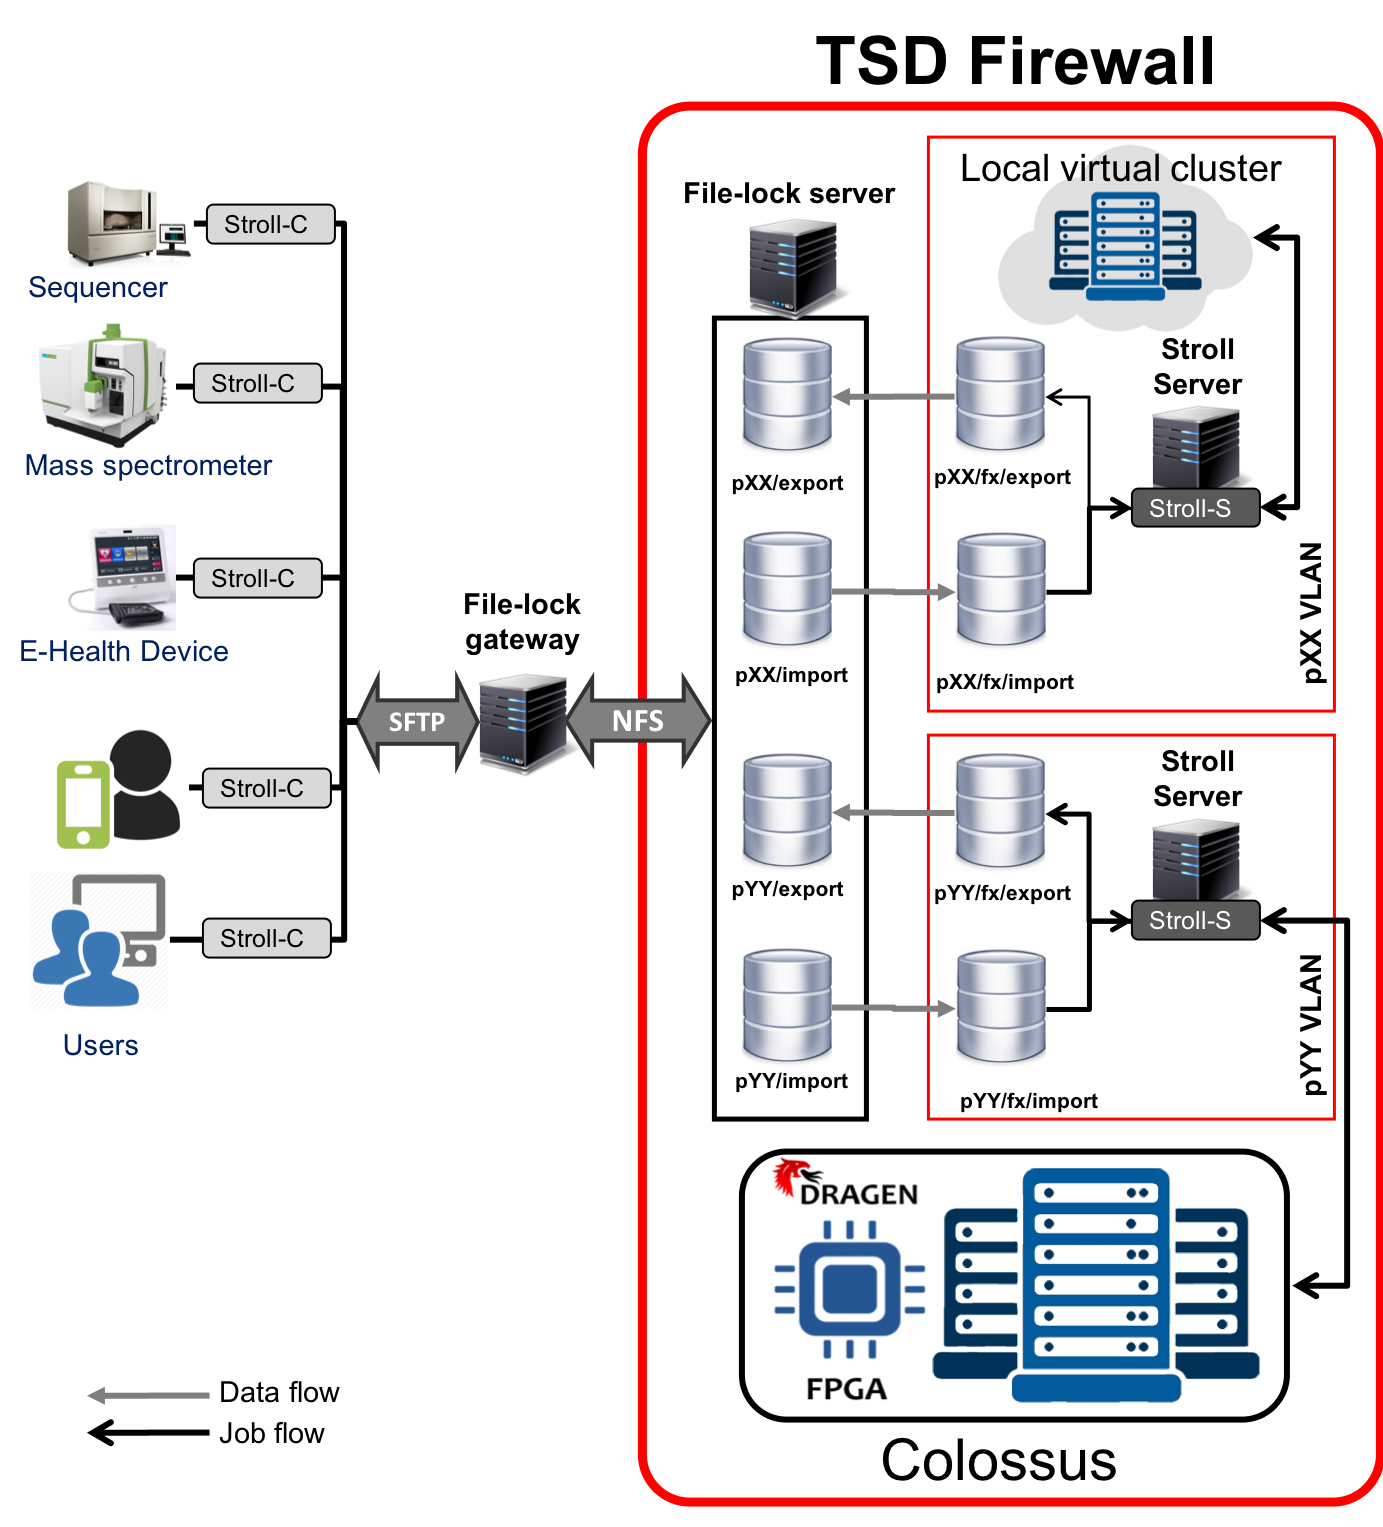
\includegraphics[width=.5\textwidth]{figures/tsd-model}                
	\caption{\name model for TSD }
	\label{fig:stroll-tsd}
\end{figure}

The external submission front-end device has \name-C component installed. The This front-end device can be: user laptop/PC, DNA Sequencer, Mass-Spectrometer, or e-health device. Each \name enabled TSD project has a dedicated VM is with \name-S installed, and read/write access enabled to the project data volume. Using this setup, the above manual steps are modified as follows:
\begin{enumerate}
	\item \textit{same as the above}
	\item The lab technician performs demultiplexing to generate FASTQ files of the sequence reads, then moves those files to a \texttt{dragen-variant-calling} directory on \name \fs, that is pre-configured as described in \secref{sec:task-structure} 
	\item In the project area, \name-S collects the job files and submits it to colossus, assigning the job to the DRAGEN node. 
	\item After the job execution is finalized on DRAGEN, \name-S exports the resulted VCF from TSD back to the hospital
\end{enumerate}

Based on this description, \name reduced the number of manual steps from five to one.



